% =====================================================================
%  Chapter 2 -- Theory
%  Every displayed equation is numbered and labelled; later chapters
%  refer back to them with \cref{eq:...}.
% =====================================================================
\chapter{Theory}\label{ch:theory}
\chapterlists

This chapter answers four questions: when does the circuit oscillate (\cref{sec:wien}); how fast does an
oscillation grow or decay near threshold (\cref{sec:growth,sec:hopf}); how late does the circuit respond
when the threshold is crossed at a finite rate (\cref{sec:sqrt-law,sec:ri-sweep}); and when does it fail
to recover under repeated crossings (\cref{sec:budget}). The symbols are collected in
\cref{tab:symbols}.

\begin{table}[!htb]
  \centering
  \footnotesize
  \renewcommand{\arraystretch}{1.08}
  \setlength{\tabcolsep}{3.5pt}
  \begin{tabularx}{\linewidth}{@{}l>{\raggedright\arraybackslash}X|l>{\raggedright\arraybackslash}X@{}}
    \toprule
    \textbf{Symbol} & \textbf{Meaning} & \textbf{Symbol} & \textbf{Meaning} \\
    \midrule
    $R$, $C$ & resistors and capacitors of the frequency-selecting (Wien) network & $G_{R}$ & sensitivity of the gain to the swept resistance, $\dd G/\dd R_{s}$ at $R_{c}$ \\
    $\RF$, $\Ri$ & feedback and input resistors that set the amplifier gain & $\lambda$ & sweep rate (\si{\ohmpersec}) \\
    $G$, $\Gc$ & amplifier gain $1+\RF/\Ri$; its oscillation threshold (ideally 3) & $t^{*}$ & delay between crossing the threshold and the visible switch \\
    $\beta$ & fraction of the output returned by the Wien network & $\Ron$, $\Roff$ & resistance at which the oscillation is seen to switch on / off \\
    $\wo$, $f_{0}$, $T_{0}$ & natural angular frequency $1/RC$, frequency $\wo/2\pi$, period $1/f_{0}$ & $k_{\mathrm{on}}$, $k_{\mathrm{off}}$ & coefficients of the $\sqrt{\lambda}$ laws (\si{\ohm^{1/2}\,\second^{1/2}}) \\
    $s$ & Laplace variable (complex growth rate) & $t_{d}$ & a fixed instrumental delay (alternative model) \\
    $v(t)$, $\Vout$ & output voltage & $X$, $R_{i,c}$, $k_{i}$ & overshoot of $\Ri$ past its threshold $R_{i,c}$; its $\sqrt{\lambda}$ coefficient \\
    $A(t)$ & envelope (amplitude) of the oscillation & $\Delta R$, $\tau$, $N$ & staircase step, time per step, number of positions \\
    $\sigma$, $\omega$ & growth rate and angular frequency of a small oscillation & $R_{k}$, $G_{k}$ & resistance and gain at staircase position $k$ \\
    $\Asat$ & saturation amplitude of the amplifier & $\Gp$, $\Gm$ & growth and decay available in one sweep cycle \\
    $\delta$ & noise floor: amplitude from which a new oscillation grows & $S_{+}$, $S_{-}$ & path sums $\sum_{k}(G_{k}-\Gc)_{+}$ and $\sum_{k}(\Gc-G_{k})_{+}$ \\
    $\Lambda$ & accumulated growth needed to go from $\delta$ to $\Asat$, $\ln(\Asat/\delta)$ & $A_{\min}$ & smallest amplitude reached in a cycle \\
    $\Lon$, $\Loff$ & growth needed for switch-on (to $90\%$), decay needed for switch-off (to $10\%$) & $\lamc$, $\lambda_{c}^{\text{(on)}}$ & critical rate for tipping to quiet; critical rate for staying on \\
    $R_{s}$, $R_{c}$ & swept resistance ($\RF$ or $\Ri$) and its threshold value &  &  \\
    \bottomrule
  \end{tabularx}
  \caption[Symbols used in the theory]{Symbols used in the theory.}
  \label{tab:symbols}
\end{table}

% ---------------------------------------------------------------------
\section{The Wien-bridge oscillator}\label{sec:wien}

\begin{figure}[!htb]
\centering
\begin{circuitikz}[font=\small]
  \ctikzset{bipoles/length=0.95cm}
  \draw (0,0) node[op amp, noinv input up] (oa) {};
  \draw (oa.out) -- ++(0.9,0) coordinate (O) node[right] {$\Vout$};
  \coordinate (N) at ($(oa.-)+(-0.5,0)$);
  \draw (oa.-) -- (N) -- ++(0,-1.1) coordinate (B);
  \draw (B) to[R, l=$\RF$, *-] (B -| O) -- (O);
  \draw (B) to[R, l_=$\Ri$] ++(0,-1.6) node[ground]{};
  \coordinate (P) at ($(oa.+)+(-2.0,0)$);
  \draw (oa.+) -- (P) node[above left, font=\footnotesize] {$V_{+}$};
  \draw (P) -- ++(0,1.4) coordinate (T);
  \draw (T) to[R, l=$R$] ++(2.0,0) to[C, l=$C$] (T -| O) -- (O);
  \draw (P) to[C, l=$C$, *-] ++(0,-1.9) node[ground]{};
  \draw (P) -- ++(-1.0,0) to[R, l_=$R$] ++(0,-1.9) node[ground]{};
  \node[font=\footnotesize, color=accent, align=center] at ($(T)!0.5!(T -| O)+(0,0.95)$) {positive feedback: selects the frequency};
  \node[font=\footnotesize, color=accent, align=center] at ($(B)!0.5!(B -| O)+(0.6,-1.0)$) {negative feedback:\\ sets the gain $G$};
\end{circuitikz}
\caption[The Wien-bridge oscillator]{The Wien-bridge oscillator. The $RC$ arms return a frequency-selected
fraction of the output to the non-inverting input; $\RF$ and $\Ri$ set the gain.}
\label{fig:wien-basic}
\end{figure}

The Wien-bridge oscillator (\cref{fig:wien-basic}) is a standard sine-wave
generator~\cite{HorowitzHill2015,SedraSmith2015,Mancini2001}; we quote the results we need. The
non-inverting amplifier has gain
\begin{equation}
  G = 1 + \frac{\RF}{\Ri} .
  \label{eq:gain}
\end{equation}
For equal resistors $R$ and capacitors $C$, the $RC$ network returns the fraction
\begin{equation}
  \beta(s) \;=\; \frac{V_{+}}{\Vout} \;=\; \frac{sRC}{(sRC)^{2} + 3\,sRC + 1}
  \label{eq:beta}
\end{equation}
of the output. It passes without phase shift at
\begin{equation}
  \wo = \frac{1}{RC}, \qquad f_{0} = \frac{1}{2\pi RC},
  \label{eq:omega0}
\end{equation}
where it returns exactly one third,
\begin{equation}
  \beta(i\wo) = \frac{1}{3} .
  \label{eq:beta-third}
\end{equation}
A signal at $\wo$ returns in phase, multiplied by $G/3$, so it grows if $G>3$ and decays if $G<3$. The
threshold is
\begin{equation}
  \Gc = 3 \qquad\Longleftrightarrow\qquad \RF = 2\,\Ri .
  \label{eq:Gc}
\end{equation}
With $R=\SI{2.17}{\kilo\ohm}$ and $C=\SI{1}{\micro\farad}$, as used throughout this work,
\begin{equation}
  \wo = \SI{460.8}{\per\second}, \qquad f_{0} = \SI{73.3}{\hertz}, \qquad
  T_{0} = \frac{1}{f_{0}} = \SI{13.6}{\milli\second} .
  \label{eq:omega0-value}
\end{equation}

\begin{whybox}[Real components]
\Cref{eq:Gc} assumes identical arms and an ideal amplifier. For a series arm $R_{1},C_{1}$ and a
parallel arm $R_{2},C_{2}$ the same analysis gives $\Gc = 1 + R_{1}/R_{2} + C_{2}/C_{1}$, so ordinary
component tolerances, together with the non-ideal amplifier, move the threshold of a real circuit away
from 3 by a few per cent. We therefore keep $\Gc$ as a symbol and measure it.
\end{whybox}

% ---------------------------------------------------------------------
\section{How fast does the oscillation grow?}\label{sec:growth}

Closing the loop requires $\Vout = G\,V_{+}$ and $V_{+}=\beta(s)\,\Vout$, i.e.
\begin{equation}
  G\,\beta(s) = 1 .
  \label{eq:loop}
\end{equation}
Substituting \cref{eq:beta} with $\wo=1/RC$ gives the characteristic equation
\begin{equation}
  s^{2} - (G-3)\,\wo\,s + \wo^{2} = 0 ,
  \label{eq:char}
\end{equation}
the Laplace form of
\begin{equation}
  \ddot{v} - (G-3)\,\wo\,\dot{v} + \wo^{2}\,v = 0 .
  \label{eq:ode}
\end{equation}
This is a harmonic oscillator with damping proportional to $(3-G)$: positive below threshold, zero at
it, negative above it. Its roots are
\begin{equation}
  s_{\pm} = \sigma \pm i\,\omega, \qquad
  \sigma = \frac{\wo}{2}\,(G-3), \qquad
  \omega = \wo\sqrt{1-\Bigl(\frac{G-3}{2}\Bigr)^{2}} ,
  \label{eq:roots}
\end{equation}
so a small signal evolves as
\begin{equation}
  v(t) = A_{0}\,e^{\sigma t}\cos(\omega t + \phi) .
  \label{eq:solution}
\end{equation}
Here $A_{0}$ and $\phi$ are the initial amplitude and phase. In our experiments $|G-3|<0.25$, so
$\omega$ differs from $\wo$ by less than $1\%$ and all the dynamics of interest is in the envelope.
Replacing 3 by the real threshold $\Gc$, the envelope $A(t)$ obeys
\begin{equation}
  \frac{\dd A}{\dd t} = \sigma A, \qquad \sigma(G) = \frac{\wo}{2}\,\bigl(G-\Gc\bigr) .
  \label{eq:sigma}
\end{equation}
For unequal arms the prefactor becomes $1/(2R_{1}C_{2})$ instead of $\wo/2$, a difference of a few per
cent for typical tolerances.

\begin{keybox}
\textbf{The rule behind everything that follows.} The amplitude changes exponentially at a rate
proportional to the distance of the gain from threshold (\cref{eq:sigma}). Near threshold $\sigma$ is
small: \emph{the circuit is slow exactly where it matters most.}
\end{keybox}

If $G$ varies in time, \cref{eq:sigma} holds at every instant and integrates to
\begin{equation}
  A(t) = A(t_{0})\,\exp\!\left[\int_{t_{0}}^{t}\sigma\bigl(G(t')\bigr)\,\dd t'\right] .
  \label{eq:envelope}
\end{equation}
The accumulated growth in the exponent is the central quantity of this report. For a staircase
sweep (the protocol of \cref{sec:protocol}) it reduces to a product of factors $e^{\sigma_{k}\tau}$, one per step of duration $\tau$.

\paragraph{A sense of scale} For $G=3.15$, $\sigma=\SI{34.6}{\per\second}$: the amplitude grows by a
factor $e$ every \SI{29}{\milli\second}, about two periods. Growing from \SI{1}{\milli\volt} to
\SI{10}{\volt} takes $\ln 10^{4}\approx 9.2$ such times, roughly a quarter of a second, and longer
closer to threshold. This is the origin of every delay that follows.

% ---------------------------------------------------------------------
\section{The Hopf bifurcation and the two states}\label{sec:hopf}

As $G$ increases through $\Gc$, the roots of \cref{eq:roots} cross into the right half-plane: the quiet
state $v=0$ loses stability and an oscillation at $\wo$ is born, a Hopf-type
instability~\cite{Strogatz2015}. Because only the saturation of the amplifier limits the amplitude, the
oscillation appears at nearly full size, rather than growing as $\sqrt{G-\Gc}$ as in a smooth
supercritical Hopf bifurcation. The growth predicted by \cref{eq:ode} stops when the output reaches
the largest voltage the amplifier can deliver. Until then the amplifier is nearly linear, so the
oscillation grows exponentially almost all the way and is clipped at an amplitude $\Asat$ that hardly
depends on $G$. The circuit therefore has two distinct states (\cref{fig:hopf}): a \textbf{quiet state},
containing only noise of size $\delta$, and an \textbf{oscillating state} of amplitude $\Asat$
(\SI{11.2}{\volt} on the bench, \SI{13.9}{\volt} in simulation). For noise floors between about
\SI{0.1}{\milli\volt} and \SI{10}{\milli\volt}, moving between the two states requires an accumulated
growth or decay of
\begin{equation}
  \Lambda \;\equiv\; \ln\frac{\Asat}{\delta} \;\approx\; 7\text{--}12 ,
  \label{eq:Lambda}
\end{equation}
which, by \cref{eq:envelope}, must be collected over time.

\begin{figure}[!htb]
  \centering
  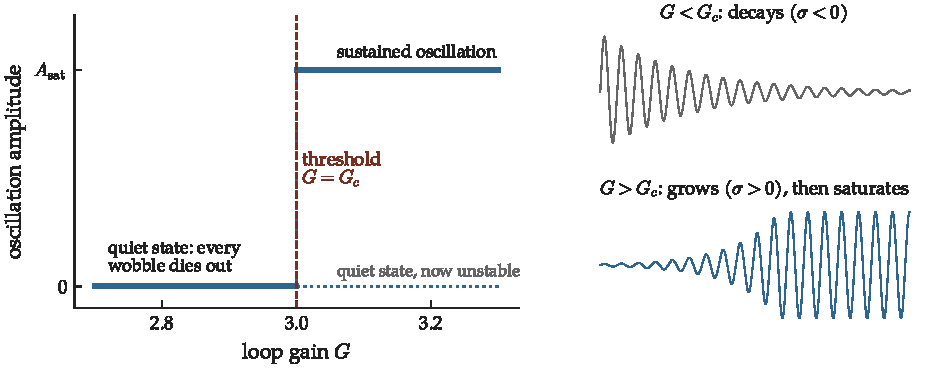
\includegraphics[width=0.85\linewidth]{fig_hopf}
  \caption[The Hopf bifurcation of the Wien-bridge oscillator]{The Hopf bifurcation. Left: quiet below
  threshold, oscillating at $\Asat$ above it. Right: response to a small disturbance on either side,
  \cref{eq:solution}.}
  \label{fig:hopf}
\end{figure}

\begin{whybox}[Why noise matters]
\Cref{eq:sigma} multiplies the amplitude already present; an exactly zero output would stay zero even
above threshold. The noise does not drive the transition but sets its starting line, and it enters only
through a logarithm: a tenfold change in $\delta$ changes $\Lambda$ by just $\ln 10\approx 2.3$.
\end{whybox}

% ---------------------------------------------------------------------
\section{Crossing the threshold at a finite rate: the \texorpdfstring{$\sqrt{\lambda}$}{square-root} law}
\label{sec:sqrt-law}

Let the swept resistance $R_{s}(t)$ pass its threshold value $R_{c}$ at $t=0$ with constant rate
$\lambda$:
\begin{equation}
  R_{s}(t) = R_{c} + \lambda t .
  \label{eq:ramp}
\end{equation}
Near threshold the gain is linear in $R_{s}$,
\begin{equation}
  G - \Gc = G_{R}\,(R_{s}-R_{c}), \qquad G_{R} \equiv \left.\frac{\dd G}{\dd R_{s}}\right|_{R_{c}} ,
  \label{eq:GR}
\end{equation}
and for a swept feedback resistor at fixed $\Ri$, \cref{eq:gain} gives exactly
\begin{equation}
  G_{R} = \frac{1}{\Ri} .
  \label{eq:GR-RF}
\end{equation}
By \cref{eq:sigma}, the growth rate then rises linearly in time:
\begin{equation}
  \sigma(t) = \frac{\wo G_{R}}{2}\,\lambda\,t .
  \label{eq:sigma-ramp}
\end{equation}

\subsection{Switching on}

Starting from the quiet state, $A(0)=\delta$, \cref{eq:envelope,eq:sigma-ramp} give
\begin{equation}
  \ln\frac{A(t)}{\delta} \;=\; \int_{0}^{t}\frac{\wo G_{R}}{2}\,\lambda\,t'\,\dd t'
  \;=\; \frac{\wo G_{R}}{4}\,\lambda\,t^{2} .
  \label{eq:logA-ramp}
\end{equation}
We call the oscillation switched on at $90\%$ of full size, which requires
\begin{equation}
  \Lon \equiv \ln\frac{0.9\,\Asat}{\delta} ,
  \label{eq:Lon}
\end{equation}
and is reached after the delay
\begin{equation}
  t^{*}_{\mathrm{on}} = \sqrt{\frac{4\,\Lon}{\wo\,G_{R}\,\lambda}} .
  \label{eq:tstar}
\end{equation}
In this time the resistor has moved $\lambda t^{*}_{\mathrm{on}}$ past threshold, so the switch-on is
seen at
\begin{equation}
  \boxed{\;\Ron = R_{c} + k_{\mathrm{on}}\sqrt{\lambda}\,, \qquad
  k_{\mathrm{on}} = 2\sqrt{\frac{\Lon}{\wo\,G_{R}}}\;}
  \label{eq:Ron}
\end{equation}
Here $\delta$ is taken as fixed. With noise acting continuously, the amplitude present at the crossing
depends weakly on the rate, so \cref{eq:Ron} is the leading-order law for switch-on; switch-off, which
starts from $\Asat$, does not have this complication.

\begin{whybox}[Why a square root?]
The accumulated growth is the area of a triangle of base $t$ and height $\sigma\propto\lambda t$
(\cref{fig:sqrt-delay}), i.e.\ $\propto\lambda t^{2}$, and it must reach the fixed value $\Lon$. Hence
$t^{*}\propto\lambda^{-1/2}$ and the overshoot $\lambda t^{*}\propto\lambda^{1/2}$: a faster ramp
switches sooner in \emph{time} but later in \emph{resistance}.
\end{whybox}

\begin{figure}[!htb]
  \centering
  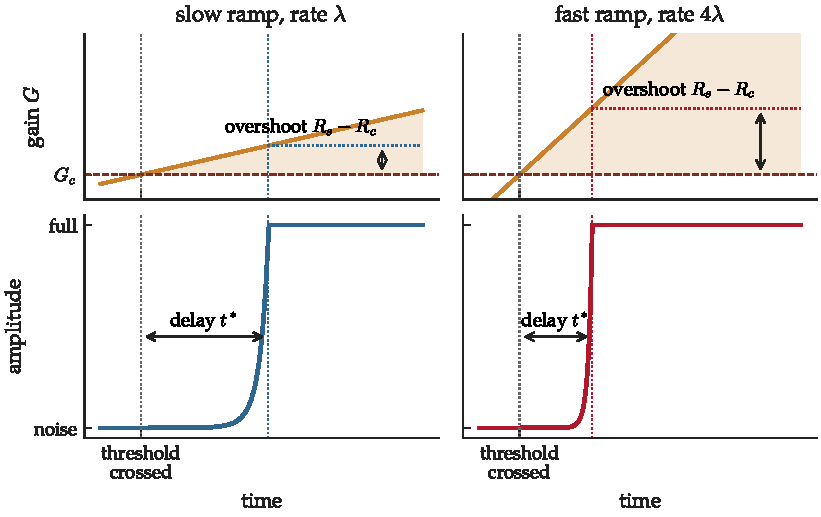
\includegraphics[width=0.85\linewidth]{fig_sqrt_delay}
  \caption[Origin of the square-root law]{Origin of the $\sqrt{\lambda}$ law: the growth collected
  (shaded, \cref{eq:logA-ramp}) must reach $\Lon$ before the amplitude leaves the noise level. A ramp
  four times faster halves $t^{*}$ and doubles the overshoot.}
  \label{fig:sqrt-delay}
\end{figure}

\subsection{Switching off}

In reverse, the gain falls through threshold with $A(0)=\Asat$. Switch-off is defined as a decay to
$10\%$, requiring
\begin{equation}
  \Loff \equiv \ln\frac{\Asat}{0.1\,\Asat} = \ln 10 \approx 2.30 ,
  \label{eq:Loff}
\end{equation}
and the same steps give
\begin{equation}
  \boxed{\;\Roff = R_{c} - k_{\mathrm{off}}\sqrt{\lambda}\,, \qquad
  k_{\mathrm{off}} = 2\sqrt{\frac{\Loff}{\wo\,G_{R}}} = 2\sqrt{\frac{\ln 10}{\wo\,G_{R}}}\;}
  \label{eq:Roff}
\end{equation}
Since the decay starts at $\Asat$ and ends at a fixed fraction of it, the noise floor never enters:
$k_{\mathrm{off}}$ is a \emph{parameter-free} prediction.

\subsection{Consequences}

\paragraph{A rate-dependent loop} Swept up and down, the circuit traces a hysteresis loop of width
\begin{equation}
  \Ron - \Roff = \bigl(k_{\mathrm{on}} + k_{\mathrm{off}}\bigr)\sqrt{\lambda} ,
  \label{eq:loop-width}
\end{equation}
which closes as $\lambda\to 0$: the loop is created by the sweep, not by the static circuit.

\paragraph{On--off asymmetry} The coefficients are in the ratio
\begin{equation}
  \frac{k_{\mathrm{on}}}{k_{\mathrm{off}}} = \sqrt{\frac{\Lon}{\Loff}} .
  \label{eq:k-ratio}
\end{equation}
Switching on is a climb from the noise floor ($\Lon\approx 9$), switching off a descent of one decade
($\Loff\approx 2.3$), so the switch-on lag should be about twice the switch-off lag.

\paragraph{The numbers} For $R=\SI{2.17}{\kilo\ohm}$, $C=\SI{1}{\micro\farad}$, $\RF$ swept and
$\Ri=\SI{47}{\kilo\ohm}$, \cref{eq:Roff,eq:GR-RF} give
\begin{equation}
  k_{\mathrm{off}} = 2\sqrt{\frac{\ln 10\times\SI{47}{\kilo\ohm}}{\SI{460.8}{\per\second}}}
  = \SI{30.6}{\ohm^{1/2}\,\second^{1/2}} .
  \label{eq:koff-value}
\end{equation}
$k_{\mathrm{on}}$ depends on $\delta$ only logarithmically: over two decades of noise it varies by about
$\pm12\%$ (\cref{tab:kon}).

\begin{table}[!htb]
  \centering
  \small
  \begin{tabular}{@{}cccc@{}}
    \toprule
    Noise floor $\delta$ & $\Lon$ (\cref{eq:Lon}) & $k_{\mathrm{on}}$ (\si{\ohm^{1/2}\,\second^{1/2}}) & $k_{\mathrm{on}}/k_{\mathrm{off}}$ \\
    \midrule
    \SI{10}{\milli\volt}  & 7.1  & 53.9 & 1.76 \\
    \SI{1}{\milli\volt}   & 9.4  & 62.0 & 2.02 \\
    \SI{0.1}{\milli\volt} & 11.7 & 69.2 & 2.26 \\
    \bottomrule
  \end{tabular}
  \caption[Predicted switch-on coefficient]{Predicted switch-on coefficient from \cref{eq:Ron} for
  $R=\SI{2.17}{\kilo\ohm}$, $C=\SI{1}{\micro\farad}$, $\Ri=\SI{47}{\kilo\ohm}$, $\Asat=\SI{13.9}{\volt}$.
  The predicted $k_{\mathrm{off}}$ is \SI{30.6}{\ohm^{1/2}\,\second^{1/2}} in every case.}
  \label{tab:kon}
\end{table}

\subsection{Why this is not simply a delay}\label{sec:not-delay}

A fixed response time $t_{d}$ of the apparatus would displace the threshold by
\begin{equation}
  \bigl(R_{s}-R_{c}\bigr)_{\text{fixed delay}} = \lambda\,t_{d} ,
  \label{eq:fixed-delay}
\end{equation}
\emph{linear} in the rate. Fitting measured thresholds with \cref{eq:Ron,eq:fixed-delay} therefore
separates the dynamics of the oscillator from the apparatus (Criterion~2).

\begin{whybox}[Terminology]
In a noise-free system the onset of oscillation after a slow Hopf passage can depend on where the sweep
\emph{started}; this memory effect is the \emph{delayed Hopf bifurcation}~\cite{Baer1989}. Our circuit
regrows from the same noise floor whenever the decay budget exceeds $\Lambda$ (regime (a) of
\cref{sec:budget}) and then keeps no such memory; the $\sqrt{\lambda}$ law is simply the consequence of
crossing a Hopf threshold at a finite rate.
\end{whybox}

% ---------------------------------------------------------------------
\section{Sweeping the input resistor}\label{sec:ri-sweep}

In Stage~4 $\Ri$ is swept with $\RF$ fixed, and $G$ is no longer linear in the swept resistance. Let
$R_{i,c}=\RF/(\Gc-1)$ be the threshold value of $\Ri$ and
\begin{equation}
  \Ri = R_{i,c} + X ,
  \label{eq:X}
\end{equation}
so that $X$ is the overshoot. Since raising $\Ri$ lowers $G$, \cref{eq:gain} gives exactly
\begin{equation}
  G - \Gc = -(\Gc-1)\,\frac{X}{R_{i,c}+X} .
  \label{eq:G-Ri}
\end{equation}
For a switch-off with $X=\lambda t$ and $A(0)=\Asat$, \cref{eq:sigma,eq:envelope,eq:G-Ri} give
\begin{equation}
  \ln\frac{\Asat}{A}
  = \frac{\wo(\Gc-1)}{2}\int_{0}^{t}\frac{\lambda t'}{R_{i,c}+\lambda t'}\,\dd t'
  = \frac{\wo(\Gc-1)}{2\lambda}\left[X - R_{i,c}\ln\!\Bigl(1+\frac{X}{R_{i,c}}\Bigr)\right] .
  \label{eq:Ri-integral}
\end{equation}
Equating this to $\Loff$ gives an exact implicit equation for the overshoot $X_{\mathrm{off}}$ at
switch-off,
\begin{equation}
  X_{\mathrm{off}} - R_{i,c}\,\ln\!\Bigl(1+\frac{X_{\mathrm{off}}}{R_{i,c}}\Bigr)
  = \frac{2\,\Loff}{\wo\,(\Gc-1)}\;\lambda .
  \label{eq:Ri-exact}
\end{equation}
Expanding $\ln(1+u)=u-\tfrac12u^{2}+\tfrac13u^{3}-\dots$ for $u=X_{\mathrm{off}}/R_{i,c}\ll 1$, the left
side becomes $X_{\mathrm{off}}^{2}/(2R_{i,c}) - X_{\mathrm{off}}^{3}/(3R_{i,c}^{2})+\dots$; solving order by
order,
\begin{equation}
  \boxed{\;R_{i,\mathrm{off}} = R_{i,c} + k_{i}\sqrt{\lambda} + \frac{k_{i}^{2}}{3R_{i,c}}\,\lambda + \dots,
  \qquad k_{i} = 2\sqrt{\frac{\Loff\,R_{i,c}}{\wo\,(\Gc-1)}}\;}
  \label{eq:Ri-off}
\end{equation}

\begin{whybox}[Meaning of \cref{eq:Ri-off}]
The leading term is \cref{eq:Roff} with $|G_{R}|=(\Gc-1)/R_{i,c}$; the curvature of \cref{eq:G-Ri} adds
a term linear in $\lambda$. For $\RF=\SI{90}{\kilo\ohm}$ and $\Gc=3$ ($R_{i,c}=\SI{45}{\kilo\ohm}$),
$k_{i}=\SI{21.2}{\ohm^{1/2}\,\second^{1/2}}$; at \SI{6}{\kilo\ohm\per\second} the square-root term is
\SI{1.64}{\kilo\ohm} and the correction only \SI{20}{\ohm}. The square-root law survives essentially
intact.
\end{whybox}

% ---------------------------------------------------------------------
\section{Repeated crossings: the growth budget}\label{sec:budget}

In the experiments a digital potentiometer steps the resistor up and down in a staircase, each step held
for $\tau$ (\cref{ch:methods}), so the threshold is crossed again and again. Here rate-induced tipping
enters.

\subsection{Growth and decay in one cycle}

Let the staircase visit $R_{k}$, $k=0,\dots,N-1$, in steps of $\Delta R$, with gain $G_{k}$. In one full
cycle every position is occupied for a total time $2\tau$, during which \cref{eq:envelope} multiplies the
amplitude by $\exp[\wo(G_{k}-\Gc)\tau]$. Separating positions above and below threshold, the growth and
decay available per cycle are
\begin{align}
  \Gp &\equiv \wo\,\tau\sum_{k}\bigl(G_{k}-\Gc\bigr)_{+} \;=\; \wo\,\tau\,S_{+} ,
  \label{eq:Gp}\\
  \Gm &\equiv \wo\,\tau\sum_{k}\bigl(\Gc-G_{k}\bigr)_{+} \;=\; \wo\,\tau\,S_{-} ,
  \label{eq:Gm}
\end{align}
with $(u)_{+}=\max(u,0)$; the sums $S_{\pm}$ depend only on the path. The staircase rate is
\begin{equation}
  \lambda = \frac{\Delta R}{\tau} ,
  \label{eq:lambda-stair}
\end{equation}
so both budgets are inversely proportional to it:
\begin{equation}
  \Gamma_{\pm} = \frac{\wo\,\Delta R\,S_{\pm}}{\lambda} .
  \label{eq:budget-rate}
\end{equation}

\begin{keybox}
\textbf{The growth budget.} Each cycle the oscillation can grow by at most $e^{\Gp}$ and shrinks by
$e^{-\Gm}$. The \emph{path} fixes their ratio; the \emph{rate} fixes their size (\cref{eq:budget-rate}).
\end{keybox}

\subsection{Three long-time behaviours}

The amplitude is confined between $\delta$ and $\Asat$, a logarithmic span $\Lambda$
(\cref{eq:Lambda}). Comparing the budgets with $\Lambda$ and with each other gives three behaviours
(\cref{fig:budget}).

\begin{figure}[!htb]
  \centering
  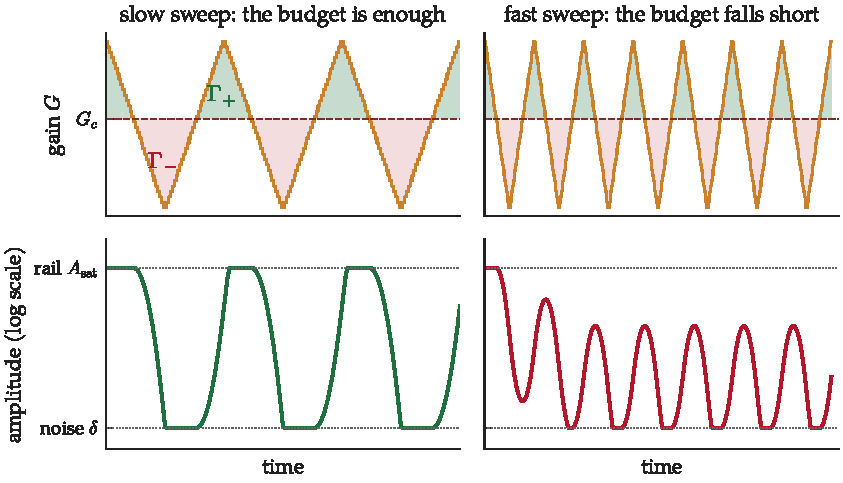
\includegraphics[width=0.85\linewidth]{fig_budget}
  \caption[The growth budget of a staircase sweep]{The growth budget. Top: the same staircase path at two
  speeds; areas above and below threshold are $\Gp$ and $\Gm$. Bottom: amplitude on a log scale. Slow: each
  pass lifts the oscillation from noise to rail. Fast: the budget is too small and the oscillation never
  climbs back.}
  \label{fig:budget}
\end{figure}

\paragraph{(a) Bursting} If
\begin{equation}
  \Gm \ge \Lambda \quad\text{and}\quad \Gp \ge \Lambda ,
  \label{eq:regime-burst}
\end{equation}
the oscillation dies to the noise floor and is rebuilt to full size every cycle: the slow-sweep regime.

\paragraph{(b) Always on} If $\Gp>\Gm$ and $\Gm<\Lambda$, the oscillation always recovers its losses
but no longer has time to die; between bursts it falls only to
\begin{equation}
  \frac{A_{\min}}{\Asat} = e^{-\Gm} .
  \label{eq:Amin}
\end{equation}
It no longer switches off (minimum above $10\%$) once $\Gm<\ln 10$, i.e.\ above
\begin{equation}
  \boxed{\;\lambda_{c}^{\text{(on)}} = \frac{\wo\,\Delta R\,S_{-}}{\ln 10}\;}
  \label{eq:lamc-on}
\end{equation}

\paragraph{(c) Tipped: off for good} If $\Gp<\Gm$ and
\begin{equation}
  \Gp < \Lambda ,
  \label{eq:tip-condition}
\end{equation}
one pass cannot lift the oscillation from noise to full size, and whatever it gains is lost on the next
pass below threshold because $\Gm>\Gp$. The circuit stays quiet in every later cycle although the gain
keeps crossing the threshold. (Slow sweeps with $\Gp<\Gm$ still burst, because the decay stops at the
noise floor and the growth budget then suffices to reach the rail.) By \cref{eq:budget-rate} this occurs
above
\begin{equation}
  \boxed{\;\lamc = \frac{\wo\,\Delta R\,S_{+}}{\Lambda}
  = \frac{\wo\,\Delta R}{\ln(\Asat/\delta)}\sum_{k}\bigl(G_{k}-\Gc\bigr)_{+}\;}
  \label{eq:lamc}
\end{equation}
Since a cycle counts as re-ignited at $90\%$ of full size, $\ln(0.9\Asat/\delta)$ would be the strictly
consistent requirement; the difference, $\ln(1/0.9)=0.11$, changes $\lamc$ by about $1\%$.

\begin{whybox}[Why regime (c) is a signature of rate-induced tipping]
Just below and just above $\lamc$ the gain visits the same values in the same order, so the frozen
circuit passes through the same sequence of states in both runs. Yet one circuit oscillates every cycle
and the other never does. Only the speed differs: this is Criterion~3, with critical rate \cref{eq:lamc}.
Each pass does cross the Hopf threshold, so this is not R-tipping in the strict sense of a stable state
that persists along the whole path (\cref{sec:what-kind}).
\end{whybox}

\subsection{Properties of the critical rates}

\paragraph{No square root} The $\sqrt{\lambda}$ laws concern one crossing, during which $\sigma$ builds up
from zero. The critical rates compare the growth of a whole pass, $\propto 1/\lambda$, with a fixed
requirement.

\paragraph{Noise} $\lamc\propto 1/\ln(\Asat/\delta)$: a noisier circuit needs less growth and tolerates
faster sweeps. Noise does not cause tipping; it sets where it occurs. \Cref{eq:lamc-on} contains no noise
term.

\paragraph{Threshold} $S_{+}$ counts only positions above threshold, weighted by distance from it; a
small shift of $\Gc$ adds or removes whole positions, so $\lamc$ is very sensitive to $\Gc$.

\paragraph{The numbers} \Cref{tab:budget-theory} gives the predictions for our two staircase paths,
taking nominal components, $\Gc=3$ and 32 positions with $\Delta R=\SI{10}{\kilo\ohm}/31$. Sweeping $\RF$
(\SIrange{91}{101}{\kilo\ohm}) puts most of the path above threshold, $\Gp>\Gm$, predicting an always-on
state above \SI{21}{\kilo\ohm\per\second}. Sweeping $\Ri$ (\SIrange{41}{51}{\kilo\ohm}) puts most of it
below, $\Gp<\Gm$, predicting tipping above about \SI{20}{\kilo\ohm\per\second} for
$\delta=\SI{1}{\milli\volt}$.

\begin{table}[!htb]
  \centering
  \small
  \renewcommand{\arraystretch}{1.15}
  \begin{tabular}{@{}lcc@{}}
    \toprule
    & \textbf{$\RF$ staircase} & \textbf{$\Ri$ staircase} \\
    \midrule
    Fixed resistor & $\Ri=\SI{47}{\kilo\ohm}$ & $\RF=\SI{90}{\kilo\ohm}$ \\
    Swept range & \SIrange{91}{101}{\kilo\ohm} & \SIrange{41}{51}{\kilo\ohm} \\
    Range of gain $G$ & 2.94 to 3.15 & 3.20 to 2.76 \\
    Positions above threshold & 22 of 32 & 13 of 32 \\
    $S_{+}$ (\cref{eq:Gp}) & 1.691 & 1.272 \\
    $S_{-}$ (\cref{eq:Gm}) & 0.329 & 2.399 \\
    Ordering of budgets & $\Gp>\Gm$ & $\Gp<\Gm$ \\
    Predicted fast-rate state & always on & tipped (off) \\
    Predicted critical rate & $\lambda_{c}^{\text{(on)}}=\SI{21.3}{\kilo\ohm\per\second}$ &
      $\lamc=\SI{19.8}{\kilo\ohm\per\second}$ for $\delta=\SI{1}{\milli\volt}$ \\
    \bottomrule
  \end{tabular}
  \caption[Growth-budget predictions for the two staircase paths]{Growth-budget predictions for
  $R=\SI{2.17}{\kilo\ohm}$, $C=\SI{1}{\micro\farad}$, $\Gc=3$, $\Asat=\SI{13.9}{\volt}$. For the $\Ri$
  staircase, $\delta=\SI{10}{\milli\volt}$ or \SI{0.1}{\milli\volt} gives $\lamc=\num{26.1}$ or
  \SI{16.0}{\kilo\ohm\per\second}.}
  \label{tab:budget-theory}
\end{table}

